\documentclass[10pt, a4paper]{article}
%-----------------------
%- 	PACKAGES & SETTINGS
%-----------------------
\usepackage[a4paper,top=1.5cm,bottom=2cm,left=4cm,right=4cm]{geometry}
\usepackage[utf8]{inputenc}
\usepackage[italian]{babel}
\usepackage{xcolor}
\usepackage{hyperref}
\hypersetup{
    colorlinks=true,
    filecolor=magenta,      
    urlcolor=darkgray,
    linkcolor=black
}
\urlstyle{same}
\usepackage{amsmath}
\usepackage{graphicx}
\graphicspath{ {images/} }
 
%-----------------------
%- 	TITLE
%-----------------------
\title{\textbf{Relazione Progetto Java PR 2}}
\author{\textbf{Venturi} Ludovico\\Docente: \href{http://pages.di.unipi.it/levi/}{Francesca Levi}}
\date{UNIPI, Novembre 2019}


%-----------------------
%- 	DOCUMENT
%-----------------------
\begin{document}
%- 	INTRO
\pagenumbering{roman} 
\maketitle
\tableofcontents
\vfill
\begin{figure}[h]
	\centering
	
\includegraphics[scale=0.1]{javaLogo}
	\label{fig:0}
\end{figure}

\clearpage

%- 	START DOC
\pagenumbering{arabic} 
\section{Scelte progettuali}
Nella relazione verranno spiegate le scelte progettuali e implementative che sono state prese.

\begin{figure}[h!]
	\centering
	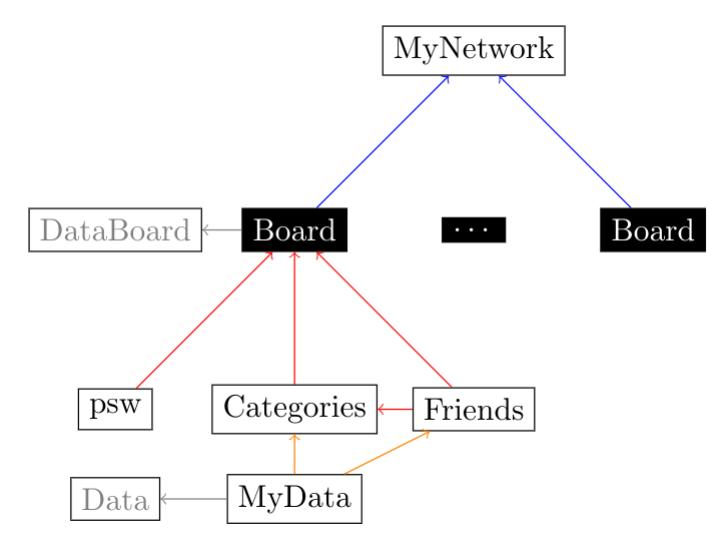
\includegraphics[scale=0.4]{diag1}
	\label{fig:diag1}
	\caption{Struttura generale del progetto (comune ad entrambe le implementazioni)}
\end{figure}

\subsection{Data}
A grandi linee è stata creata una struttura generale dei dati in grado di adattarsi a varie situazioni.\\ \texttt{Data} viene implementata come \textit{interfaccia}: stabilisce un \textit{contratto} con le sottoclassi che la implementeranno. 
\begin{center}
OVERVIEW: \textit{Data rappresenta un dato astratto sottoforma di un insieme di 2 attributi e alcune operazioni. È una struttura astratta immutable, di dimensione finita e fissa}
\end{center}
Stabilisce delle caratteristiche comuni a tutte le sottoclassi: metodi che dovranno necessariamente implementare: 
\begin{center}
\texttt{public void \emph{display}();\\public String \emph{getDataTitle}();\\public 		String \emph{getCategory}();}
\end{center}
\subsubsection{MyData}
Viene poi implementata una sottoclasse \textit{astratta \texttt{MyData}} per soddisfare l'obiettivo iniziale di progettare una struttura versatile.\\
\texttt{MyData} è implementata come classe astratta e tale scelta deriva dalla volontà di attribuire a tutte le classi che discendono da \texttt{MyData} delle altre caratteristiche comuni, più \textit{concrete}, ovvero dei metodi già implementati e una struttura implementativa di base:
\begin{center}
	\texttt{private String \emph{dataName};\\
	private String \emph{category};\\}
\end{center}
Come da specifica la classe \texttt{MyData} riporta anche il metodo display, ma astratto: verrà implementato dalle sottoclassi.
Da \texttt{MyData} discendono i dati veri e propri che saranno salvati in bacheca: nell'esempio per il progetto sono \texttt{Testo} e \texttt{Audio}, che:
\begin{itemize}
	\item ridefiniscono \texttt{equals()} per permettere la deep equality
	\item aggiungono un contenuto
	\item implementano \texttt{display()}
\end{itemize}

\subsubsection{Ipotesi}
\begin{itemize}
	\item La bacheca risulta una collezione di oggetti di vario tipo, come riportato nel testo, ma ciò non è direttamente collegato ad \texttt{«E extends Data»}. Si è pertanto deciso di riportare anche la classe (magari apparentemente superflua) \texttt{MyData} in modo da far trasparire chiaramente la presa di coscienza di ciò. La bacheca gestisce collezioni di dati di tipo E : pertanto ogni dato sottotipo di E, con E definito come \texttt{«E extends Data»}, è un dato valido da inserire in una bacheca basata sul tipo E (l' \texttt{upcasting} è sempre possibile in queste condizioni); nel progetto si creano bacheche di tipo \texttt{MyData} e vengono caricate con dati di tipo \texttt{Audio} e \texttt{Testo}, entrambi sottotipi di \texttt{MyData}
	\item Non ci sono setter poichè si è ipotizzato che \textit{Data} fosse una struttura \textit{immutable}.\\
	\begin{footnotesize}
(Nel testo viene riportato «\textit{i dati possono essere
visualizzati dagli amici ma modificati solamente dal proprietario della bacheca}»: ciò è stato interpretato come: "la modifica consiste nell'aggiunta o la rimozione dei dati, non nella  modifica effettiva del contenuto dei dati").
\end{footnotesize}
 \end{itemize}
 

\bigskip
\subsection{Board«E extends Data» }

\texttt{Board} rappresenta un contenitore di oggetti generici. È basata sul tipo generico \texttt{«E extends Data»} e funzionalmente è una collezione di dati che possono essere di vario tipo, a patto che siano sottotipi di E (che estende \texttt{Data}).

Non ho riportato la specifica di ogni metodo nel codice di \texttt{Board(2)«E extends Data»} poichè risultava troppo confusionario; l'implementazione ha comunque seguito di pari passo la specifica riportata nell'interfaccia \texttt{DataBoard«E extends Data»}.
\subsubsection{Ipotesi}
\begin{itemize}
\item non sono ammessi elementi \texttt{null}
\item non sono ammessi duplicati di alcun genere
\item il numero di likes non dipende solamente dal dato ma anche dalla bacheca in cui si trova $\Rightarrow$ \texttt{MyData} o le sue sottoclassi non possiedono il contatore dei like: questo si trova nella bacheca, relativamente ad ogni dato
\item la lista ritornata da \texttt{getDataCategory} è in sola lettura, avendo precedentemente ipotizzato che Data sia immutable
\item la rimozione di una categoria comporta la perdita dei dati in quella categoria e l'associazione per ogni amico di quella categoria
\item i likes sono univoci per ogni amico
\item \texttt{get()} ritorna il dato vero e proprio, non una copia, ma ciò non crea problemi poichè è stato scelto di rendere i dati \textit{immutabili}
\item la rimozione della condivisione di una categoria con un amico non comporta la rimozione dei like che quest'ultimo ha assegnato ai vari dati di quella categoria
\item ad un dato è associata una e una sola categoria
\end{itemize}
\paragraph{Nota sugli Iteratori} Gli Iteratori sono stati implementati come classi \textit{interne} alla classe \texttt{Board}, precisamente come classi di \textit{istanza}. Non sono \textit{static} poichè dipendono dal tipo generico \texttt{E} e devono accedere alle variabili di istanza.\\ Implementano l'interfaccia \texttt{Iterator«E»}; non implementano il metodo \texttt{remove()}, anzi sollevano un' \texttt{UnsupportedOperationException} se chiamato.\\
Quando invocati gli iteratori restituiscono un iteratore di istanza della classe interna (la quale, si ricordi, ha visibilità limitata a \texttt{Board}). \\
Ad esempio: 
\begin{center}
	\texttt{public Iterator«E» \emph{getFriendIterator}(String friend)}
\end{center}
quando 	invocato ritorna un'istanza della classe interna:
\begin{center}
	\texttt{private class \emph{FriendIterator} implements Iterator«E» }
\end{center}
che implementa i metodi \texttt{hasNext()} e \texttt{next()} e che gestisce al suo interno una struttura dati contenente i dati su cui iterare:
\begin{itemize}
\item nel caso di \texttt{getFriendIterator} vengono salvati su una struttura di supporto tutti i dati delle categorie condivise con quell'amico
\item nel caso di \texttt{getIterator} vengono salvati su una struttura di supporto \textit{tutti} i dati in bacheca, dispendioso, ma necessario per poter applicare un ordinamento crescente in base ai like (data la struttura in cui sono memorizzati normalmente). Per gestire questo iteratore è stata creata una nuova classe interna \texttt{private class \emph{LikeSortedDataIterator} implements Iterator«E»}.
\end{itemize}
\paragraph{Gestione delle Password} Si è scelto di salvare le password tramite \texttt{hash} in array di \texttt{byte}\footnote{https://www.baeldung.com/java-password-hashing}, il tutto è gestito nella classe \texttt{public final class \emph{MyPasswordCrypt}}.
\paragraph{Eccezioni} Sono stati documentati tutti i sollevamenti delle \texttt{eccezioni}. In più sono state definiti 3 nuovi tipi di eccezione: \texttt{DuplicateLikeException, HiddenCategoryException, WrongPasswordException} tutte sottoclassi di \texttt{RuntimeException} e quindi \textbf{unchecked}.
\subsubsection{Implementazione 1}
Per la prima implementazione di \texttt{Board} è stata scelta la seguente struttura: 
\begin{center}
\texttt{private HashMap<String, ArrayList<InternalData<E>>> \emph{categories}\\
	private HashMap<String, ArrayList<String>> \emph{friends}}
\end{center}
con \texttt{InternalData<E>}  definito come segue: 
\begin{center}
\texttt{E data\\
		ArrayList<String> friendsWhoLiked\\
		int likes}
\end{center}
La scelta di utilizzare \texttt{HashMap«K,V»} è stata basilare in modo da poter avere associazioni univoche per chiave, e accessi veloci alla struttura. 
Rimangono però da gestire le chiavi duplicate (non accettabili qui) e/o \texttt{null} (ne ammette 1) così come si deve garantire che i valori inseriti nella \texttt{HashMap} non siano mai \texttt{null}. \\
\texttt{ArrayList«E»} è stato scelto poiché di semplice utilizzo come contenitore di una quantità variabile di elementi. Si deve far attenzione a non inserire elementi \texttt{null} o duplicati.\\
\texttt{InternalData«E»} è un \textit{record} interno alla classe \texttt{Board} usato per poter gestire l'associazione \textsc{dato-like} e valgono le stesse considerazioni per l' \texttt{ArrayList} (utilizzato al suo interno) degli altri sopra.

\subsubsection{Implementazione 2}
Per la seconda implementazione di \texttt{Board} è stata scelta la seguente struttura: 
\begin{center}
\texttt{private HashMap<String, TreeSet<InternalData<E>>> \emph{categories}\\
	private HashMap<String, TreeSet<String>> \emph{friends}}
\end{center}
con \texttt{InternalData<E>} che utilizza \texttt{TreeSet<String> \emph{friendsWhoLiked}}
al posto di \texttt{ArrayList}, e pertanto valgono le stesso considerazioni precedenti più quelle sotto per il \texttt{TreeSet} utilizzato al suo interno.\\
Per \texttt{HashMap} valgono le stesse considerazioni dell'implementazione 1.\\
\texttt{TreeSet} è stato scelto per le sue proprietà molto interessanti: non ammette \texttt{null}, non ammette duplicati e salva i dati in ordine crescente. Nonostante questo sono stati comunque effettuati alcuni controlli sui parametri poiché necessari per altre operazione che non riguardavano un \texttt{TreeSet}.
Da notare che per far sì che il \texttt{TreeSet} comparasse a dovere il tipo \texttt{InternalData«E»} è stato definito un comparatore interno alla classe \texttt{Board}. Nell'iteratore invocato in \texttt{getIterator()} l'utilizzo del TreeSet ha permesso di evitare l'ordinamento di tutti i dati.
Per scorrere ogni \texttt{TreeSet} si è abbondantemente fatto uso degli \texttt{iteratori}.
\section{Eseguire il codice}
Eseguendo il \texttt{main} si può testare la struttura già presente che testa tutte le funzionalità.
È riportata la prima implementazione di \texttt{Board}, per testare la seconda è sufficiente \textsl{fare un find and replace di \texttt{" Board"} con \texttt{" Board2"} (spazi compresi)}.
\subsection{Test ed esempi}
Nel \texttt{main} sono già presenti un insieme di operazioni che testano il progetto. \\
Viene creata una \texttt{rete} in cui sono presenti 2 bacheche di 2 utenti e, oltre a funzionare, mostra principalmente come vengono gestite le eccezioni. In generale più istruzioni in un singolo blocco \texttt{try-catch} indicano che l'ultima sarà quella che genera l'eccezione mentre le precedenti sono eseguite con successo.\\
Non saranno verificati \textit{tutti} i casi in cui parametri sono null per ovvie ragioni, così come tutte le eccezioni ripetute, quali i controlli che la categoria esista o che l'amico sia presente nella lista amici; per queste ultime, pur se generabili in differenti occasioni, verranno esplicitamente testate una volta ciascuna. 
Lista di test effettuati nel \texttt{main}:
\begin{enumerate}
\item password della bacheca « 8 caratteri
\item get di una bacheca non presente
\item password errata
\item stringa nulla passata (vale per tutti i metodi)
\item aggiunta di una categoria già presente
\item rimozione di una categoria non presente
\item condivisione di una stessa categoria con uno stesso amico
\item condivisione di una categoria non presente nella bacheca
\item rimozione di un amico non presente nella lista amici
\item rimozione di un amico da una categoria cui non ha accesso, anche se presente nella lista amici
\item inserimento di un dato già presente
\item inserimento di un dato la cui categoria non è presente in bacheca
\item get di un dato la cui categoria non è presente
\item get di un dato non presente
\item get di un dato precedentemente inserito in modo corretto ma la cui categoria è stato poi rimossa
\item rimozione di un dato non presente
\item getDataCategory e modifica della lista ritornata
\item amico vuole inserire like ad un dato di una categoria non condivisa con lui
\item amico vuole inserire like ad un dato cui lo ha già messo
\item amico vuole inserire like ad un dato non presente
\item ITERATORI, prove varie
\item elimino una categoria e itero sui dati di tale categoria tramite una amico con cui essa era condivisa
\end{enumerate}

\end{document}
